\documentclass[journal,twoside]{IEEEtran}

\usepackage[utf8]{inputenc}
\usepackage[T1]{fontenc}
\usepackage{microtype}

\usepackage{amsmath}

\usepackage{tabularx}
\usepackage{booktabs}
\renewcommand{\arraystretch}{1.3}

\usepackage[sorting=none, style=ieee]{biblatex}
\addbibresource{biblio.bib}
\renewcommand*{\bibfont}{\footnotesize}

\usepackage{graphicx}
\graphicspath{{images/}}

\hyphenation{op-tical net-works semi-conduc-tor}

\title{Classification of Images Using a Neural Network}

\author{Group 20: Indraj \textsc{Gandham}, Jakub \textsc{Grzmil}, Babar \textsc{Khan}, Jack \textsc{Longmuir},\\ Ben \textsc{Storrs}, Charles \textsc{Stubbs}}

\markboth{Intelligent Systems 2 (INT2) Open Group Assessment}%
{Gandham \MakeLowercase{\textit{et al.}}: Classification of Images Using a Neural Network}

\usepackage{lipsum}

\begin{document}
\maketitle

\begin{abstract}
The task is to design and implement a machine learning model which can classify the images from the CIFAR-10 test set into ten distinct categories. We did this by designing and implementing a convolutional neural network (ConvNet) with six 2D layers, employing ReLU as the loss function. We trained our ConvNet using the CIFAR-10 training data for 110 epochs (total training time was 22 minutes). The classification error our ConvNet achieved on the CIFAR-10 test set was 19.56\%.
\end{abstract}

\section{Introduction}
\IEEEPARstart{F}{or this} project, our team will be designing and implementing a neural network in order to classify images using the CIFAR-10 image dataset. We will train our network to recognise different categories of images provided by the dataset, so that, when provided with a 2D image input, the network will be able to classify said image into the correct category.

In 1982, British neuroscientist David Marr created a low-level algorithm to detect edges, curves and corners in the image. Around  the same time, Japanese computer scientist Kunihiko Fukushima created a self-organising artificial network which could detect patterns using convolution called Neocognition. Both of these individuals were inspired by the works of David Hubel and Torsten Wiesel in 1959 who, at the time, were trying to determine how cats perceived images. They noticed that when a new image was slid into the projector, a single neuron fired; this led to the discovery that visual processing always starts with simple structures such as orientated edges.

Modern approaches for image processing came from the Imagenet challenge. Since 2012, only convolution-based networks have won the challenge, dropping the error rate in previous years from $\sim{}20\%$ down to only a few percent. \cite{demush:vision}

Image classification is an important machine learning problem with a range of modern applications; for example, in facial recognition software and in self-driving cars (to identify pedestrians walking across the road).

In this project, we will be leveraging the PyTorch framework to implement a convolution-based neural network, performing training and testing with the CIFAR-10 dataset.

\begin{figure*}[t!]
\centering
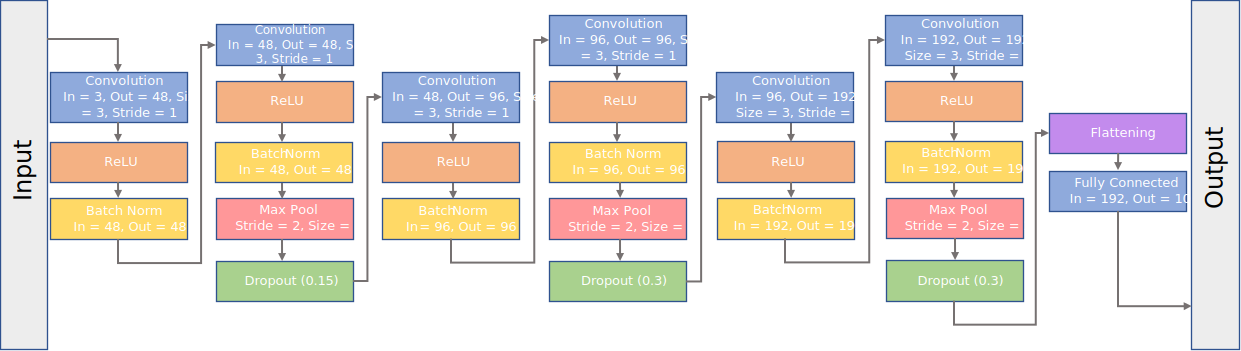
\includegraphics[width=\textwidth]{diagram.pdf}
\caption{Diagram showing network architecture.}
\end{figure*}

\section{Method}
This section describes the process of our image classifier, explaining the inner workings and technical details of our neural network.

The neural network consists of six 2D convolutional layers, each with their own individual kernels (kernel size~$=3$, i.e. $3\times{}3$, using a stride of 1), with our first 2D convolutional layer taking three input channels from the image (one for red, one for green and one for blue) and outputting 48 convolutional features to the second 2D convolutional layer, which takes those 48 convolutional features from the first layer, applies a similar process and outputs another 48 convolutional features. The following four convolutional layers take 48, 96, 96 and 192 input channels and output 96, 96, 192 and 192 convolutional features respectively. Each of these convolutional layers output their convolutional features to our ReLU activation function (discussed later), which is followed by batch normalisation and max pooling stages (with the exception of our first, third and fifth layers, which operate without a max pooling stage and therefore do not reduce the matrix representation of our image in size). We chose a kernel length of 3 for the convolutional layers because this enables padding to be added to both sides, ensuring that the image remains centred and unaltered. Each of these convolutional layers is optimised for our use case by the presence of sparse connections -- this helps us reduce our number of parameters, which increases training speeds. We also utilise a constant filter, whereby the same weights are used for each convolutional operation (further reducing our number of parameters).

The output of each convolution layer is passed to the ReLU function, which is a non-linear activation function (we also do this following the pooling layers, discussed later). ReLU returns its argument whenever it is greater than 0, and returns a value very close to 0 otherwise (this is to avoid impact on learning). The ReLU function is shown in Equation~\ref{eq:relu} and leaky ReLU (as implemented) is shown in Equation~\ref{eq:leaky_relu}.

\begin{align}
f\left(x\right)&=\text{max}\left(0,x\right) \label{eq:relu} \\
f\left(x\right)&=\text{max}\left(0.01x,x\right) \label{eq:leaky_relu}
\end{align}

ReLU is very useful because it has many of the desirable properties of a linear activation function when training the neural network using backpropagation, but still enables non-linear learning as negative values always yield 0. Without applying ReLU as part of our neural network, we would essentially just have a linear regression model. As such, it is key to apply non-linear transformation to our inputs.

Our six convolutional layers and their corresponding applications of ReLU are followed by a batch normalisation stage, whereby a process of standardisation is undertaken on our inputs as part of each mini-batch. This process of batch normalisation effectively means that assumptions made by a given subsequent layer within the neural network around the spread and distribution of our inputs do not change dramatically, which helps to stabilise and increase the speed of its learning. Applying this process enabled us to reduce the number of epochs from around 700 to 120. Following the universally applied stage of batch normalisation across our convolutional layers is the occasionally applied stage of max pooling (again, with the exception of our first, third and fifth layers), with this process being employed to reduce the number of parameters in our model by utilising downsampling. Downsampling enables the model to detect features in a manner that is more robust to object orientation or scale changes -- essentially, we widen the size of our `window' to cover more pixels, and then take the statistical maximum over the contents of that window, before placing the output result into a new matrix (the model uses a kernel size of $2\times{}2$ and a stride of 2 for our `widened window', with default padding and dilation). This new matrix is then fed forwards to the next convolutional or fully connected layer, and the process is repeated with or without a max pooling stage depending on which of the six ordinal convolutional layers are invoked. The final output matrix from the network's terminal max pooling layer is handed to the fully connected layer (preceded by ReLU application and batch normalisation).

The final stage of the deep neural network is the fully connected layer. The role of the fully connected layer is to sort the output from the preceding layers into useful, predefined categories that can be used to classify the contents of the image and provide a logical, user-friendly output (one of ten available image categories). Our fully connected layer takes 192 in-features and transforms these into 10 out-features by utilising PyTorch's \texttt{Linear} class, essentially reducing and flattening all of its input channels into a single tensor of order $n\times{}1$. We can use this tensor to extract a corresponding category, and use that category to display a classification output.

The overall model error is calculated by our cross-entropy loss function. We aim to optimise our loss function by minimising its error output, making use of stochastic gradient descent in order to attain the best possible classification accuracy. We chose the cross-entropy loss function because it is widely used to measure the performance of models that output probabilities between 0 and 1, which aligns with our objectives. Once an iteration of the model has been completed, the neural network runs through a process of backpropagation in order to adjust the weights in between our layers, which will (over time) bring us closer to our goal of a minimal classification error.

\newpage

\section{Results \& Evaluation}

\begin{table}[h!]
\label{table:results}
\caption{Results from testing different hyperparameters}

\begin{tabularx}{\columnwidth}{llX}
\hline
Epochs & Batch Size & Accuracy\\
\hline
2 & 10,000 & 10\% \\
10 & 64 & 34\% \\
50 & 64 & 52\% \\
100 & 64 & 62\% \\
110 & 50 & 80\% \\
\hline
\end{tabularx}
\end{table}

We calculated the accuracy of our model by dividing the number of correct classifications in the test batch by the total number of test images and multiplying by 100 to get a percentage. The optimisation algorithm we used was stochastic gradient descent, with a momentum of 0.9 and a learning rate of \texttt{1e-3} for epochs under 80, \texttt{1e-3/2} for epochs under 120, \texttt{1e-3/3} for epochs under 200 and \texttt{1e-3/4} for higher epochs. We chose this optimisation algorithm because it results in faster learning compared to other options as an update is performed after each data instance is processed.

We tested a number of different parameters and hyperparameters before arriving at our final accuracy. First we experimented with adjusting the number of epochs and the batch size. With 2 epochs and a batch size of 10,000 we got an accuracy of 10\%. Increasing the number of epochs to 10 and decreasing the batch size to 64 gave us an accuracy of 34\%. Further increasing the number of epochs to 50 while keeping the batch size at 64 gave us an accuracy of 52\%, and doubling the number of epochs to 100 with the same batch size of 64 gave us an accuracy of 62\%.

We then decided to experiment with different numbers of layers, with combinations of 3 to 6 convolution layers and 1 to 3 linear layers, and batch sizes of 32, 50, 64 and 1024. 1024 specifically batches ended up performing very badly so we used lower batch sizes going forward, 50 to be exact as that gave the best accuracy in the earlier experiments. We also experimented with using drop out layers with values of 0.1, 0.25 and 0.5. After this we attempted to lower the learning rate as we increase epochs; specifically we divided it by 10 after 15 epochs and then after 30 epochs we further divided it by 40, which increased the accuracy to 69.59\%. We then decided to use batch normalisation, which decreased the number of epochs required to reach our maximum accuracy from 700 to about 120.

Our final accuracy was 80.44\% which was achieved at 110 epochs after 22 minutes, more specifically the neural network classified 8,044 images correctly out of a test sample of 10,000. This was the highest accuracy that we managed to achieve with our neural network and one with which we were satisfied given our low accuracies of around 10\% with the first experiments. This is also an accuracy at which the neural network has some practical use in non-critical applications. The hardware environment used was an Nvidia RTX 3070 GPU (with 5888 CUDA cores), an AMD Ryzen 5 3600 CPU, 16GB of 3200MHz RAM and a Gigabyte Aorus Elite x570 motherboard.

\section{Conclusion \& Further Work}
Overall, we believe that our model performed well on the CIFAR-10 test set. There is a table on Wikipedia detailing the error rates of research papers claiming state-of-the-art results \cite{wiki:cifar}; the error rate of our model was 19.56\%, which places it between Convolutional Deep Belief Networks on CIFAR-10 \cite{krizhevsky:belief} and Maxout Networks \cite{goodfellow:maxout}, which had error rates of 21.1\% and 9.38\% respectively. This supports our conclusion about our model's performance.

We believe that our architecture was a good choice because we achieved a low classification error in a short period of time (total training time was only 22 minutes).

For this project, the testing phase of hyperparameters went rather well. This enabled us to go from what was 10\% accuracy with a batch size of 10,000 to changing the number of epochs, mini-batches, etc. to get us to our final accuracy of 80.44\%.

One area that didn't go as well was the normalisation of the data -- at first, we were doing this incorrectly, causing us to take more time training the network. One thing to perhaps work on in the future, is to try a cyclical learning rate to find a good initial starting point. This is because although our learning rate changes as it goes our initial learning rate was manually chosen.

\printbibliography[heading=bibintoc]

\end{document}

